%!TEX program = xelatex
\documentclass[varwidth,border=0pt]{standalone}

\usepackage{fontspec}
\setmainfont{Times New Roman}

% the various libraries we will be using
\usepackage{tikz}
\defaultfontfeatures{Ligatures=TeX}

% define colours
% taken from pickton on Adobe Kuler:
% https://kuler.adobe.com/Some-Kind-Of-Execushares-color-theme-3837185/
\definecolor{ExecusharesRed}{RGB}{230,37,52}
\definecolor{ExecusharesBlack}{RGB}{43,40,40}
\definecolor{ExecusharesBlue}{RGB}{22,190,207}
\definecolor{ExecusharesWhite}{RGB}{255,255,243}
\definecolor{ExecusharesGrey}{RGB}{107,110,108}

\begin{document}
	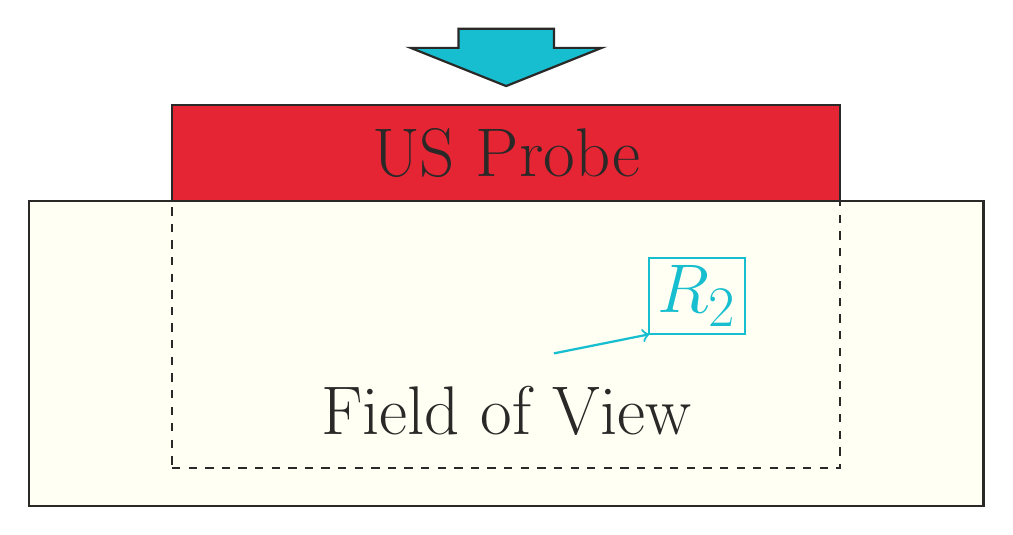
\begin{tikzpicture}[x=\textwidth,y=0.4\textwidth]
		\draw[thick, draw=ExecusharesBlack, fill=ExecusharesWhite]
		(0, 0) -- (1, 0) -- (1, 0.8) -- (0, 0.8) -- cycle;
		\draw[dashed, thick, draw=ExecusharesBlack, fill=none]
		(0.15, 0.1) -- (0.85, 0.1) -- (0.85, 0.8) -- (0.15, 0.8) -- cycle;
		\draw[thick, draw=ExecusharesBlack, fill=ExecusharesRed]
		(0.15, 0.8) -- (0.85, 0.8) -- (0.85, 1.05) -- (0.15, 1.05) -- cycle;
		\draw[thick, draw=ExecusharesBlack, fill=ExecusharesBlue]
		(0.5, 1.1) -- (0.6, 1.2) -- (0.55, 1.2) -- (0.55, 1.25) -- (0.45, 1.25) -- (0.45, 1.2) -- (0.4, 1.2) -- cycle;
		\draw[thick, draw=ExecusharesBlue, fill=none]
		(0.65, 0.45) -- (0.75, 0.45) -- (0.75, 0.65) -- (0.65, 0.65) -- cycle;
		\tikzset{text=ExecusharesBlue}
		\node at (0.7, 0.55) {\fontsize{28}{28}\selectfont $R_2$};
		\draw[thick, ->, draw=ExecusharesBlue, fill=ExecusharesBlue]
		(0.55, 0.4) -- (0.65, 0.45);
		\tikzset{text=ExecusharesBlack}
		\node at (0.5, 0.925) {\fontsize{28}{28}\selectfont US Probe};
		\tikzset{text=ExecusharesBlack}
		\node at (0.5, 0.25) {\fontsize{28}{28}\selectfont Field of View};
	\end{tikzpicture}
\end{document}